\documentclass[pdftex, a4paper,11pt, oneside]{article}


\usepackage{styles/style}
\usepackage{booktabs}
\usepackage{float}
\usepackage{subfig}
\usepackage{tabularx}

\newcommand{\ra}[1]{\renewcommand{\arraystretch}{#1}}
%\usepac
\newcommand{\code}[1]{{\small\texttt{#1}}}

\begin{document}

\title{Objetos Puros observables y transaccionales. \\
Con Monitoreo de transacciones}
\author{Ronny De Jesús}

\begin{titlepage}
\begin{center}

% logo de la universidad.

\includegraphics{img/logo_unq}\\

\ \\ % force an empty line
% textsc is small caps
\textsc{
\huge
Universidad Nacional de Quilmes\\
\Large
Tecnicatura en Programación Informática\\
\ \\
Trabajo de inserción profesional\\
\rule{\linewidth}{0.2mm} %linea
}
 

\textsc{\huge  \bfseries
Objetos Puros observables y transaccionales \\
Con Monitoreo de transacciones\\}

\vfill
\vfill

\begin{tabular}{ccc}
	\emph{Alumno} &  \emph{Director} & \emph{Co-Director}\\
	{\Large Ronny De Jesús } &  {\Large Ing. Nicolás Passerini} & {\Large Ing.
	Javier Fernándes}\\
	\EmailURL{nnydjesus@gmail.com} & \EmailURL{npasserini@gmail.com} &
	\EmailURL{javier.fernandes@gmail.com}
\end{tabular}

\vfill % fill vertical space
%
% Bottom of the page
Abril 2012
%
\end{center}
\end{titlepage}


\tableofcontents{}
\newpage

\listoffigures{} % indice de figuras
\newpage

\begin{abstract}


Al desarrollar interfaces de usuario, con frecuencia gran parte del tiempo se
destina pocas tareas rutinarias, como el traspaso de datos entre los objetos
del dominio y los componentes de la interfaz gráfica. Si bien esta tarea es
simple, cuando su realización es manual la vuelve propensa a errores.
Adicionalmente, muchas interfaces de usuario requieren la posibilidad de que el
usuario cancele la operación que está realizando. En una aplicación
multiusuario, las tareas para garantizar consistencia ante una cancelación no
son sencillas. En este trabajo se propone una posible solución a estos
problemas basada en programación orientada a aspectos. Un primer aspecto
permite que los objetos de dominio en forma transparente disparen eventos al
ser modificados, de forma de actualizar la interfaz de usuario acorde a esos
cambios. Un segundo aspecto automatiza las operatoria relacionada con las
cancelaciones, permitiendo que las modificaciones a los objetos del dominio se
realicen siguiendo el concepto de transacción, y concentrándonos en las
propiedades de atomicidad y consistencia.

\end{abstract}



\section{Introducción}

Este trabajo tiene por objetivo automatizar dos tareas comunes en el
desarrollo de aplicaciones orientadas a objetos.

La primera de estas tareas es el traspaso de datos entre los objetos del dominio
y los componentes de la vista, en el contexto de la creación de interfaces de
usuario siguiendo el patrón \emph{MVC}.
 
La segunda tarea es proveer un mecanismo que permita deshacer cambios que se
hubieran realizado como parte de una operación que se comenzó y que no se puede
o no se desea finalizar.
En el contexto de la programacion orientada a objetos, estas operaciones son
modificaciones en el estado de un objeto.
Por ejemplo, si un usuario cancela una operación desde
la interfaz o si se produce una excepción durante la ejecución, la aplicación
debe garantizar que todos los objetos afectados se devuelvan al estado que
tenían antes de comenzar la operación inconclusa.

\medskip 

En este trabajo se propone una posible solución a estos problemas, basada en
\emph{programación orientada a aspectos}.
Un primer aspecto, llamado \emph{Observable} (POO), permite que, en forma
transparente, los objetos de dominio disparen eventos al ser modificados.
De esta forma la interfaz de usuario puede actualizarse y reflejar esos
cambios en forma automática.

Un segundo aspecto, llamado \emph{Transaccional} (POT), automatiza la
cancelación de una operación, garantizando que todos los objetos quedan en el
mismo estado en el que estaban antes de comenzar. 
Esto permite que las modificaciones a los objetos del dominio se realicen
en forma \emph{transaccional}, en particular las propiedades de
\emph{atomicidad} y \emph{consistencia}.

Para desarrollar POT y POO se construyó una herramienta llamada
\emph{Aspects for Pure Objects} (APO).
APO es una herramienta para programacion orientada a aspectos que abstrae
conceptos fundamentales y complejos del framework \emph{Javassist}. 
APO es independiente de POT y POO, se puede utilizar
para la creación de otros aspectos.

Para mostrar la posibilidad de componer los aspectos POO y POT se los integró en
una extensión del framework \emph{Arena}.
Arena es un framework educativo para la creacion de interfaces de usuario
utilizado.
Las extensiones desarrolladas en el marco de este trabajo han sido incorporadas
a la última versión del Arena que ya está siendo utilizada en la materia de
Construcción de Interfaces de Usuario de la Universidad Nacional de Quilmes,
entre otras.

\bigskip

\subsection{Estructura de este trabajo}
\noindent Este trabajo consta de las siguientes secciones:

\begin{itemize}
	\item {\bf Contexto}\\
		En la Sección \ref{Context} se introducen algunos de los conceptos básicos que
		son necesarios para la compresión del trabajo.
	\item {\bf Estado del Arte}\\
		En la Sección \ref{StateOfTheArt} se describen las estrategias más comunes
		utilizadas actualmente en la industria para solucionar atacados por este trabajo.
	\item{\bf Objetivo y Solución}\\
		La Sección \ref{Objective} detalla el objetivo de este trabajo y la Sección
		\ref{Solucion} describe la estrategia propuesta para alcanzarlo.
	\item{\bf Implementación y Ejemplo}\\
		Las Secciones \ref{Implementacion} y \ref{Example} describen la
		implementación de la herramienta y proveen ejemplos de utilización de la misma.
	\item{\bf Conclusiones y Trabajo futuro}\\
		En las Secciones \ref{Conclusions} y \ref{Futurework} se detallan las
		conclusiones del trabajo y y posibles caminos para continuarlo.
\end{itemize}

\subsection{Construcción de interfaces de usuario usando el patrón MVC}
	\subsubsection{MVC}
	El patrón \emph{Modelo-Vista-Controlador} (MVC) es una forma de construir
	interfaces de usuario (UI) que propone dividir el comportamiento de una
	aplicación en tres partes \cite{reenskaug79}:
		\begin {itemize}
		\item {\bf Modelo}
			El modelo representa nuestra percepción del mundo real. 
			Maneja el comportamiento y la información del dominio de la aplicación,
			responde a los pedidos de información sobre su estado y tiene la
			responsabilidad última de llevar a cabo el comportamiento del sistema.
			
		\item {\bf Vista}
			La vista tiene la responsabilidad de interactuar con el usuario, es la
			parte más fácil de identificar ya que es la que vemos en pantalla.
			La comunicación con el usuario es bidireccional:
			por un lado le muestra información proveniente del modelo y por el otro lado
			recibe acciones de parte del usuario, que representa internamente como eventos.
			
		\item {\bf Controlador}
			Es el intermediario entre el modelo y la vista.
			Captura los eventos emanados de ambos y coordina la interacción entre los
			dos.
	\end {itemize}
	 
	La idea principal de MVC, y que influyó a la mayoría de los frameworks de
	presentación posteriores, es la de Presentación Separada \emph{(Separated
	Presentation)} \cite{burbeck87}.
	Esto nos brinda una clara separación de responsabilidades entre interfaz,
	lógica de negocio y control. Además nos permite soportar múltiples
	presentaciones para un mismo modelo de información.
	La figura \ref{mvc} muestra las relaciones entre los tres componentes.  
	
	\begin{figure}[h]
		\centering
		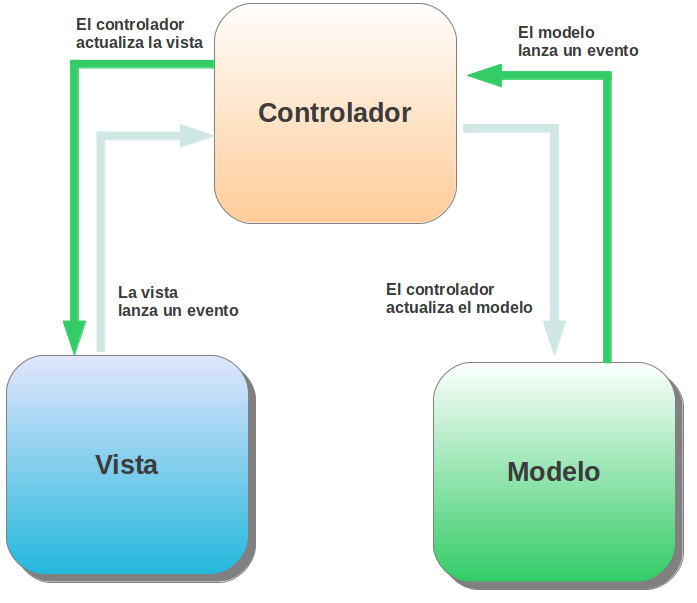
\includegraphics[width=300px, height=300px]{img/mvc} 
		\caption{Esquema MVC}
		\label{mvc}
	\end{figure}  
	
\subsubsection{Eventos}
\label{Eventos}

		Un evento es un suceso en el sistema, como una interacción del usuario con
	la máquina, o un cambio en el estado interno de un objeto.
	En un sistema orientado a eventos, existen fuentes que producen eventos y
	\emph{listeners} que se registran para ser notificados de esos eventos y poder
	actuar en consecuencia.	
	El patrón \emph{Observer} \cite{Gamma1995} es una forma común de implementar la
	idea de evento en lenguajes orientados a objetos.
	
	\begin{quote}
	
	\begin{description}
	   
	\item [Objetivo] Definir una dependencia 1:n de forma que cuando el objeto
		1 cambie su estado, los n objetos sean notificados y se actualicen
		automáticamente, a estos objetos se los conoce como \emph{listener}. Esto me
		permite una comunicación entre objetos con muy bajo acoplamiento.
	
	\item [Motivación] En la construcción de interfaces de usuarios, se tiende
		a separar los objetos de presentación (vistas) de los objetos de dominio, de
		forma que se puedan tener varias vistas sincronizadas de la misma información.
	
	\end{description}
	\end{quote}
	
\subsubsection{Binding}
\label{binding}

	El \emph{binding} es una conexión entre dos \emph{propiedades} de dos objetos, que
	permite mantener sincronizado el valor de una propiedad en el primer
	objeto con el valor de alguna propiedad en el segundo objeto.
	Habitualmente esto se logra a través del uso de eventos.
	
	Una \emph{propiedad} es una característica que el objeto exhibe hacia su exterior, 
	permite consultar su valor y en algunos casos también actualizarlo.
	Normalmente la implementación no será una variable de instancia, sino un mecanismo de más alto nivel.
	Por ejemplo, en el lenguaje Java las propiedades siguiendo el contrato denominado JavaBeans, 
	que especifica que un objeto que tenga la propiedad \code{nombre} 
	debe proveer implementaciones para los mensajes \code{getNombre} y (opcionalmente) \code{setNombre}.
	
	En la construcción de interfaces de usuario es habitual utilizar el concepto de
	binding para sincronizar los datos que está viendo o modificando el usuario
	con la información contenida en el modelo.
	Cada vez que el usuario ingresa o modifica un valor en la pantalla, la
	vista dispara un evento indicando el cambio de ese valor. Todas las
	propiedades del modelo que estén conectadas con esa propiedad, serán
	actualizadas automáticamente.
	Esto permite que el modelo tome acciones en función de la información ingresada por el usuario, 
	por ejemplo validarla y rechazarla en caso de ser incorrecta.
	En caso que las dos propiedades no sean del mismo tipo, el binding provee
	estrategias para realizar las conversiones que fueran necesarias.
		
	\bigskip

	El binding provee una estrategia de muy alto nivel para comunicar información entre
	los objetos de dominio y los componentes de la vista.
	En entornos sin binding, resolver esta problemática suele requerir gran
	cantidad de trabajo, incrementando los tiempos de desarrollo y la probabilidad
	de que ocurran errores en tareas repetitivas.
	Por ejemplo, es posible que mientras se está mostrando el valor de una
	propiedad en pantalla, algún otro proceso en curso modifique el valor de esa propiedad; 
	si no contamos con una herramienta
	para automatizar la actualización de la información mostrada en
	pantalla, la pantalla quedará desactualizada y mostrará al usuario información incorrecta.

	\medskip

	Este trabajo se enfoca en bindings \emph{bidireccionales}, es decir, aquellos
	que permiten que el flujo de información vaya en ambos sentidos: si el
	modelo cambia se actualiza la vista y si la vista cambia se actualiza el
	modelo.
	Para que esto sea posible tanto el modelo como la vista deben disparar eventos 
	cada vez que cambie el valor de alguna de sus propiedades.
	
	La necesidad de que los objetos de dominio disparen eventos plantea un problema
	si (como en muchos casos) no tenemos soporte del lenguaje para eso.
	La implementación de eventos más habitual mediante un patrón observer (\ref{Eventos}), 
	implica agregarle responsabilidades a los objetos de dominio que no tienen que ver con
	el dominio en sí. Genera más burocracia, ensucia la interfaz y obliga a meter
	lógica para disparar eventos, mezclado con la ejecución de la acción de
	negocio. En definitiva violar el MVC por sí mismo no es algo malo, lo malo son
	las consecuencias que eso trae.
	
	Otro problema que aparece frecuentemente es que el binding modifica los objetos
	directamente, al menos en su versión más sencilla. 
	Esto significa que cada vez que el usuario ingresa un valor en la pantalla,
	se modifica el objeto de dominio asociado, aún cuando la navegación de la aplicación podría
	permitirle al usuario cancelar la operación que está realizando.
	En caso de cancelarse la operación, los cambios realizados sobre los objetos
	deben deshacerse para retrotraer el objeto al estado que tenía al comenzar la
	operación. Implementar este proceso en forma manual es una tarea repetitiva y
	por lo tanto propensa a que ocurran errores por parte del programador.
	
\subsubsection{Framework Arena}
	Arena es un framework para la construcción de interfaces de usuario. 
	Esta creado con fines educativos y por lo tanto se focaliza en la puesta en
	práctica de algunos principios de diseño y organización de
	interfaces de usuario.
	El framework fue diseñado e implementado por el equipo docente de la materia de
	Construcción de Interfaces de Usuario de la Tecnicatura Universitaria en Programación
	Informática de la Universidad Nacional de Quilmes, en conjunto con docentes de
	la Universidad de San Martín y de la Facultad Regional Buenos Aires de la Universidad Tecnológica Nacional.
	
	 
\subsection{Transacciones}	

Una transacción es una unidad en la ejecución de un programa que se comporta 
\emph{atómicamente}: debe ejecutarse por completo o fallar sin dejar rastro, no
puede dejar los datos en un estado intermedio.

Los objetivos de trabajar con transacciones son dos.
En primer lugar, definir unidades de trabajo seguras, que permitan 
recuperarse de los errores y mantener la coherencia de los datos, incluso en caso de fallas en el sistema.
En segundo lugar, permitir el acceso concurrente, es decir, que múltiples
usuarios utilicen la misma información al mismo tiempo sin interferir entre sí.

\medskip
Para poder trabajar con transacciones se deben contar con instrucciones
especiales para marcar su inicio y su final:
\begin{quote}
	\label{ctxTransactional}
	\begin{description}
		\item[Begin transaction] es una operación que marca el inicio de una
		transacción. Toda operación que se haga de aquí en más quedará en suspenso
		mientras dure la transacción.
	
		\item[Commit] es una operación que finaliza y confirma los
		cambios realizados desde el inicio de la transacción. 
		
		\item[Rollback] es una operación que finaliza y revierte todos los cambios
		realizados desde el inicio de la transacción, 
		dejando los datos en el estado que tenían antes de comenzar.
	\end{description}
\end{quote}
   
\bigskip

Muchas veces las transacciones se asocian con los sistemas de gestión de bases
de datos, sin embargo es un concepto más general.
Por ejemplo, en interfaces de usuario es común incluir botones de
``aceptar'' y ``cancelar'' que podemos relacionar con las ideas de
\emph{commit} y \emph{rollback}. 
Si el usuario presiona el botón ``cancelar'' lo que se espera
es que los datos de la aplicación queden en el estado exacto en el que estaba
antes de comenzar la tarea.

\bigskip
\label{sec:ACID}
Para garantizar la integridad de los datos, se considera que un sistema de
transaccional debe cumplir con un conjunto de propiedades denominadas por el
acrónimo \emph{ACID} \cite{HaerderReuter83}.
De las propiedades ACID, este trabajo se concentra en las de \emph{Atomicidad},
\emph{Consistencia} y \emph{Aislamiento}. 

\begin{description}
	\item[Atomicidad]
		Una operación en un sistema de software se considera \emph{atómica} cuando se
		puede garantizar que no se realizará parcialmente aún cuando ocurran errores
		durante su ejecución. 
		En caso de operaciones complejas que constan de varias sub-operaciones, si una
		de las sub-operaciones no se puede completar, ninguna de las sub-operaciones
		debe ejecutarse. Si se detecta una falla después de que una de las
		sub-operaciones ya fue realizada, se debe deshacer dicha
		sub-operación, garantizando que el sistema vuelva al estado original antes de
		comenzar la operación.
		
	\item[Consistencia]
		Un sistema transaccional se considera que cumple con la propiedad de
		\emph{consistencia} si existe una forma de garantizar la integridad de los
		datos cada vez que termina una transacción.
		En programación orientada a objetos, el encapsulamiento permite que cada
		objeto se ocupe de su propia consistencia. 
		Entonces, una estrategia para lograr consistencia es evitar que otras partes
		de la aplicación manipulen los datos del dominio por fuera de los
		propios objetos de dominio.
	  
	\item[Aislamiento] \label{isolation}
		Para cumplir la propiedad de \emph{aislamiento}, ninguna
		transacción debe interferir con la ejecución de otra transacción.
		Es una práctica común considerar diferentes \emph{niveles de aislamiento}
		\cite{ANSI:1992:ANSd}, que miden el grado de independencia que tienen dos
		transacciones ejecutándose al mismo tiempo.

		Las técnicas propuestas en este trabajo intentarán alcanzar el nivel
		denominado \emph{Read committed}.
		En este nivel solo se pueden ver los datos que están confirmados, es decir, si
		una transacción esta haciendo una modificación, esta no es visible a otra
		transacción hasta que sea confirmada.

% 	\item{\bf \emph{Read uncommitted}}
% 				Este es el menor nivel de aislamiento. En él se permiten las lecturas
% 				sucias, es decir, una transacción pude ver cambios no confirmados
% 				aún por otra transacción.]

% 		A continuación se listan los niveles de aislamiento que presentan mayor
% 		interés en este trabajo:
% 		
% 		\begin{description}
% 			\item []
% 				
% 		  \item [Serializable]
% 				Este es el nivel de aislamiento más alto. Especifica que todas las
% 				transacciones ocurran de modo aislado, o dicho de otro modo, como si todas las
% 				transacciones se ejecutaran secuencialmente, es decir, una tras otra. 
% 			\end{description}
	
	\end{description}
		

\subsection{Programación orientada a Aspectos}

	La programación orientada a aspectos (POA) es un estilo de programación cuyo
	principal objetivo es mejorar la  separación entre los requerimientos
	funcionales de los no funcionales, para ganar expresividad, disminuyendo la
	dispersión del código asociado a un concepto y haciendo que las
	implementaciones resulten más comprensibles, adaptables y reutilizables.


\subsubsection{Definición de un Aspecto}
	Según el trabajo seminal de Gregor Kiczales y otros, un aspecto es 
	``una unidad modular que se disemina por la estructura de
	otras unidades funcionales. Los aspectos existen tanto en la etapa de
	diseño como en la etapa de implementación. Un aspecto de diseño es
	una unidad modular que se entremezcla en la estructura de otras partes
	del diseño. Un aspecto de programa o de código es una unidad modular
	del programa que aparece en otra unidades del programa.'' \cite{Kicz97a}

	\bigskip
	
	Un aspecto es la unidad básica de construcción en la POA, debido a que permite
	modularizar los conceptos transversales o \emph{cross-cutting concern} presentes en una aplicación.
	
	En palabras simples un aspecto puede ser definido como: ``La encapsulación y
	modularización de un \emph{cross-cutting concern}''. Por ejemplo en las  
	
	La definición de un aspecto se basa en los conceptos de: {\bf \emph{Join
	Point}}, {\bf \emph{ Point Cut}} y {\bf \emph{ Advice}}.
	
	\begin{quote}
	
	\begin{description}
		\item[\emph{Join Point}] Un \emph{Join Point} puede ser definido como un punto
		en la ejecución de una aplicación, como por ejemplo: la creación de una instancia, el manejo de una
		excepción, una llamada a un método, el retorno de un método, la asignación de
		un valor a una variable, etc.
		
		\item[\emph{Point Cut}] Un \emph{Point Cut} hace referencia a un conjunto de
		Join Point que cumplen cierta condición, es decir, permiten exponer el contexto de
		ejecución de dichos \emph{points}.
		
		\item[\emph{Advices}] Y por último los \emph{Advices}, éstos pueden definirse
		como: acciones que se ejecutan en cada \emph{Join Point} dentro de un mismo
		\emph{Point Cut}, estas acciones se traducen en rutinas o fragmentos de
		código.
	
	\end{description}
	\end{quote}
	
	



\section{Estado del arte}
\label{sec:StateOfTheArt}


\subsubsection{Eventos}

1) a mano (Arena actual | SWT | javabeans)
2) wicket => web
				bind con submit
		Desventajas
			se pierden validaciones del lado del dominio
			concepto del form
3) investigar que hace morphic




\subsubsection{Transacciones}

(Buscar implementaciones o soluciones | proyectos)

1) clonar
2) aplication model
3)transacciones de DB
\section{Objetivo}
\label{Objective}
El primer objetivo de este trabajo es automatizar la comunicación entre el
modelo y la interfaz de usuario.
Toda vez que el usuario ingrese información en el sistema, la
información debe llegar directamente hasta el dominio. Esto nos permite
aprovechar toda la lógica del dominio durante la edición.
De la misma forma, si cambia un atributo de un objeto de dominio, se debe
informar a la UI para que ese cambio sea visible
inmediatamente.
Toda esta funcionalidad debe poder ser implementada en forma transparente,
sin modificar el dominio ni imponerle restricciones.

El segundo objetivo es proveer un soporte para transacciones, que
permita automatizar el \emph{rollback} en la operación en curso que no se pueda
finalizar o que el usuario decida cancelarla.
Además, dos usuarios deberán poder trabajar con la misma información
simultáneamente con un grado de aislamiento \emph{read committed}.

El tercer objetivo es proveer una sistema de monitoreo para las transacciones,
que permita ver el estado de todas las transacciones actuales, y una descripción
sobre los objetos y los atributos que están afectados por la transacción.

\section{Solución propuesta}
\label{Solucion}

	Basándonos en el paradigma AOP modelamos como aspectos dos conceptos: {\bf Observable} y  {\bf Transaccional}.
	En las secciones subsiguientes se describe el comportamiento de cada uno de
	estos dos aspectos y en la sección \ref{sec:Union} la integración de ambos.

	\subsection{Aspecto Observable}
	\label{aspectoObservable}
		El aspecto Observable implementa un mecanismo transparente para que cuando un
		objeto de dominio cambia, cualquier parte del sistema pueda recibir una
		notificación informando ese cambio.
		Para ello, el sistema permite asociar a cada propiedad de un objeto un conjunto de \emph{listeners}. 
		El aspecto intercepta modificación a una propiedad
		de un objeto observado y notifica a los listeners que se han registrado para observar esa propiedad.
		
		Este mecanismo permite asociar acciones específicas que se disparan cada vez
		que el objeto es modificado. En particular, se utiliza para mantener
		sincronizada la UI con los objetos del dominio.

	\subsection{Aspecto Transaccional}
	\label{aspectoTransaccional}
		El aspecto transaccional permite controlar la visibilidad de las modificaciones
		realizadas a un objeto.
		Llamamos \emph{objeto transaccional} a los objetos a los que se les aplica este aspecto.
		
		Para controlar la visibilidad de las modificaciones realizadas sobre los objetos transaccionales, 
		se define el concepto de \emph{contexto transaccional}.
		Un contexto transaccional es un espacio de trabajo en el cual se pueden
		realizar operaciones que no serán visibles fuera de ese contexto.
		Toda acción realizada dentro del sistema es asociada con algún contexto transaccional.
		
		El aspecto transaccional intercepta \textbf{en forma transparente} todos los accesos al
		estado interno de los objetos transaccionales, permitiendo la intervención del contexto.
		Cuando se modifica el estado interno de un objeto transaccional el nuevo valor es almacenado en el contexto y 
		el objeto permanece inalterado.
		Cuando se desea leer el estado interno de un objeto transaccional se toma el valor del contexto, en caso de existir.
		De esta manera las operaciones realizadas dentro del mismo contexto ven un estado del objeto que es distinto 
		al que ven las operaciones realizadas en cualquier otro contexto.
	
		Los contextos transaccionales se delimitan por las
		operaciones detalladas en la Sección \ref{ctxTransactional}
		(\emph{beginTransaction}, \emph{commit} y \emph{rollback}).
		La operación de \emph{commit} confirma las modificaciones y las hace públicas
		fuera del contexto.
		Por su parte, la operación de \emph{rollback} provee un
		mecanismo automático para descartar todas las modificaciones realizadas
		dentro del contexto.
		Al ejecutarla, todos los objetos modificados dentro del contexto regresan al
		estado que tenían al comenzar la transacción.
		 
		El contexto transaccional permite el trabajo concurrente, de esta forma
		varias operaciones dentro de un mismo sistema pueden acceder a un objeto transaccional al mismo
		tiempo con un aislamiento de nivel \emph{read commited}.
				 
		También se da soporte para \emph{transacciones anidadas}, es decir, la
		posibilidad de abrir un nuevo contexto transaccional dentro de otro contexto,
		denominado \emph{contexto padre}.
		Esta funcionalidad permite dividir una transacción en partes que pueden ser
		revertidas o confirmadas individualmente.
		
	\subsection{Integración de ambos aspectos entre sí y con la UI}
	\label{sec:Union}
		Al utilizar ambos aspectos simultáneamente aparecen situaciones complejas que
		deben ser tenidas en cuenta. También es necesario estudiar la forma en que
		puedan integrar ambos aspectos con la UI.
		Para atacar estos problemas se tomaron tres acciones:
		
		\begin{enumerate}
		  \item Cuando la UI muestra en pantalla el valor de una
		  propiedad de un objeto de dominio, debe registrarse como listener de esa
		  propiedad.
		  De esa forma, en caso de producirse un cambio en el valor de la propiedad, la
		  UI podrá reflejar esa modificación en forma inmediata.
		  
		  \item Siempre que desde la UI el usuario tenga la posibilidad de cancelar
		  una acción que comenzó a realizar, se debe utilizar un contexto
		  transaccional.
		  Esto se logra incluyendo en la UI las operaciones de
		  \emph{beginTransaction}, \emph{commit} y \emph{rollback}.
		  
		  Consideramos que la decisión de cuándo comenzar o terminar una transacción 
		  no puede ser decidida por nuestro framework de transacciones. 
		  La estrategia utilizada para integrar un framework
		  específico de UI con el aspecto transaccional es extender el framework
		  elegido con herramientas que manejen los contextos transaccionales en forma
		  automática.
		  
		  \item La integración de los aspectos entre sí se logra asociando a
		  cada listener con un contexto transaccional y limitando el alcance de los
		  eventos producidos por el aspecto observable para que sólo notifiquen a los
		  listeners que se encuentran en la mismo contexto transaccional que produjo el cambio.
		\end{enumerate}

\section{Aplicación de ejemplo}
(Fijarse si se puede poner en la problemática)\\
1)Edición con cancelar\\
2)múltiple cancelaciones\\
3)buscador\\
4)monitor de transacciones\\

Para comprender mejor esta problemática veamos un ejemplo. Supongamos una simple
aplicación bancaria, donde los clientes de un banco pueden transferir dinero de
una cuenta a otra. Al realizar un transferencia, hay que extraer el monto
indicado de la primera cuenta, y depositarlo en la segunda. Estas dos
operaciones pueden tener errores, como por ejemplo, extraer un monto mayor al
saldo, o depositar mas cantidad de la maxima permitida.

La  figura \ref{example} muestra el diagrama de la aplicación de
ejemplo

	\begin{figure}[h]
		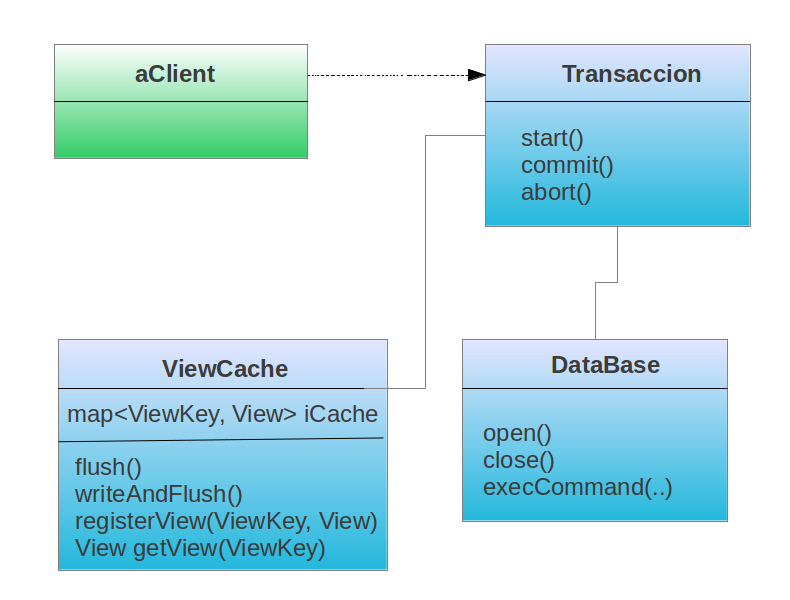
\includegraphics{img/objectTransaction}
		\caption{Diagrama UML de la aplicación de ejemplo}
		\label{example}
	\end{figure}	


El sistema me permite 

\section{Nuestra herramienta: }

Con el propósito de cumplir el objetivo detallado en la Sección
\ref{sec:Objetivo} y llevándolo a cabo con la solución propuesta en la  la
Sección \ref{sec:Solucion}, se desarrolló dos conceptos \emph{Pure Objects
Observable} (POO)  para atacar a la problemática de la observabilidad y
\emph{Pure Object Transaction} (POT) para atacar a la problematica
transaccional.

\medskip  

Se evaluaron dos frameworks para resolver nuestro problema. Uno es Javassist y
el otro AspectJ. \cite{KiczalesHHKPG01}

\medskip 

Se utilizó Javassist porque es independiente al usuario, en cambio si utilizamos
AspectJ obligamos al usuario a el compilador del código. 

\medskip 

Ya que Javassist es muy de bajo nivel, y trabaja a nivel de \emph{bytecode},
trajabar con el es complicado y el codigo se hace intendible. Por eso se
desrrollo una herramienta llamada \emph{ Aspect for Pure Object} (APO), que es 
una abstracción del Framework Javassist, que permite fácilmente implementar un
aspecto, y aplicarselo a un grupo de objetos.

\comment{Hay ciertos parametros en la aplicación que son configurables. Para
ello hay que editar el archivo \emph{framework-config.properties}}.

\medskip 

Utilizando \emph{APO} se implementaron los dos aspectos diferentes:

	\subsection{Aspecto Transaccional (POO)} 
		Esta basado en una implementación
		hecha por Nicolás Passerini y Javier Fernandes.
		 
		Utilizando la programación orientada a aspectos, intercepta todas las lecturas
		y escrituras de los \emph{fields}. Insertando código al momento de la carga de
		la clase.
		Se remplaza el acceso al field, tanto de lectura como escritura, y se lo delega
		al ObjectTransactionManager, donde se guarda la información en una estructura
		[objeto, [Field, Valor]].
		
		\medskip
		
		El contexto de la transacción esta asociado a un solo \emph{tread}. Esto
		permite manejar la concurrencia en el acceso a la información de los objetos. 
		Soportando transacciones anidadas, donde cada transacción hija hereda el estado
		de su padre, y al momento de hacer el \emph{commit} en la sub-transacción, sus
		cambios son impactados en la transacción padre.
		Por esta forma de implementación, la identidad del objeto se mantiene, ya que
		el objeto no se modifica ni se clona, solo se cambia el acceso a sus fields.
		
		Para agregarle este aspecto a una clase se utiliza la \emph{Annotation}
		\emph{Transactional }
		
			\begin{lstlisting} 
				@Transactional
				public class Client extends Entity {
				}
			\end{lstlisting}

	\subsection{ Aspecto Observable}
			
		En su implementación interna lo que hace el aspecto es agregar un \emph{field
		changeSupport} del tipo \emph{<<PropertySupport>>} al objeto que se va a
		convertir en Observable. Pero su implememtacion se optiene del el archivo de
		configuracion con la \emph{key: framework.aop.poo.changeSupport}.
		Luego se agrega métodos para completar su objetivo.
		El primero es el \emph{firePropertyChange} que es el que notifica a los
		Observadores que una propiedad ha cambiado.	Luego le agregamos
		\emph{addPropertyChangeListener} y \emph{removePropertyChangeListener} para
		poder agregar y remover Observadores para que escuchen sus cambios.
		
		Para agregarle este aspecto a una clase se utiliza la \emph{Annotation}
		\emph{Observable}
		
			\begin{lstlisting} 
				@Observable
				public class Client extends Entity {
				}
			\end{lstlisting}
		


\subsection{Integración de ambos aspectos } 
	Framework me permite poder tener uno u otro , o
	ambos aspecto. Se puede poner los dos \emph{Annotation} \emph{Observable} y
	\emph{Transactional} como vimos previamente, o ponerle uno solo. 
	
	\begin{lstlisting} 
		@TransactionalAndObservable
		public class Client extends Entity {
		}
	\end{lstlisting}
	
	
	
\subsection{Integración de aspectos con el Arena}
	En Arena se integró los dos aspectos, el Observable y el transaccional, con el
	fin de que los objetos de dominio sean puros, y que no tengan la noción de
	eventos, ni transacciones, y así poder bindearlos con los componentes de de la
	interfaz gráfica. Y al cancelar la edición poder revertir los cambios
	transparéntenme.
	
	Para ello se tubo que asociar una transacción con una ventana, en el caso mas
	especifico con la clase \emph{TransactionalDialog}. A su vez también tenemos
	vinculado los eventos del dominio junto con la ventana y la transacción.
	Se implemento tres niveles de aislamiento de los eventos,  \emph{Fire All},
	\emph{Fire Committed} y \emph{Fire olnly in my transaction};
	
	\begin{description}
		\item[\emph{Fire All}] Todos los eventos disparados por el dominio son
		escuchados, sin importar si están en una transacción.
	
		\item[\emph{Fire Committed}] Solo se escucha los eventos de las transacciones
			comiteadas
		
		\item[\emph{Fire olnly in my transaction}] solo se escucha los eventos que
			ocurren dentro de su translación.
	
	 \end{description}
	 
	 \medskip
	 
	\subsubsection{Monitor de Transacciones}
	
	 Con arena también se desarrolló un {\bf Monitor de Transacciones}, que me
	 muestra el estado actual de la transacción, incluyendo las transacciones
	 anidadas. Mostrandome los objetos afectados por la transacción y que
	 propiedades se modificaron.
	 
	 
 

	
\subsection{Buscar un  titulo}
La implementación de la integración en el arena se realizó con Scala, agregando
mejora al Arena como: Árboles, Listas \ldots \ldots \ldots. 
	
	
Contar que esta publicado, con la licencia y blah

Test de los aspectos



\section{Conclusiones}
\label{Conclusions}
Hoy en día existe gran cantidad de herramientas para el
desarrollo de UI. Sin embargo algunos problemas que son muy habituales en los desarrollos
industriales no son resueltos adecuadamente por dichas herramientas.
Cuando esto sucede, los programadores deben recurrir a soluciones
\emph{ad-hoc},  que muchas veces implican atacar problemas generales de forma
manual y escribiendo grandes cantidades de código rutinario, que con
frecuencia resulta propenso a errores.

En este trabajo abordamos dos problemas rutinarios de las UIs:
por un lado la sincronización de datos entre la vista y el modelo de dominio; y
por otro la posibilidad de modelar operaciones que se realicen atómicamente.

%lo pudimos hacer y quedó algo piola
Utilizando las ideas de la programación orientada a aspectos pudimos desarrollar
una herramienta que soluciona ambos problemas en forma \emph{transparente}, dado
que no requiere que hagamos modificaciones en el código del dominio, y \emph{genérica},
dado que es aplicable a un gran conjunto de posibles dominios.

%pruebas, cómo nos convencemos de que lo que hicimos sirve
\medskip

Para poner a prueba el aspecto transaccional, se lo aplicó en una aplicación de
mayor tamaño que los ejemplos mostrados en este trabajo.
Para eso se desarrolló la aplicación de un kiosco, escrita en su totalidad en
Scala y utilizando el framework Swing de Java para la UI.
Este desarrollo además nos permite comprobar que los aspectos están desacoplados
entre sí y pueden ser utilizados independientemente del framework Arena.

% otras cosas útiles
%Apo

Por otro lado, para dar soporte al desarrollo aprovechando el aspecto transaccional, 
se desarrolló un sistema de monitoreo para las transacciones.
Este sistema permite visualizar las transacciones, proveyendo una interfaz que muestra los
objetos afectados por la transacción.

\medskip

%utilidad en la docencia.
Finalmente, los aspectos transaccional y observable fueron integrados al framework Arena, 
favoreciendo su uso para la enseñanza de construcción de interfaces de usuario.
En las versiones previas los estudiantes tenían que disparar los eventos en forma
manual, y eso implicaba explicar conceptos complejos, distrayendo la atención de
los temas fundamentales de la materia.

Como resultado adicional de este trabajo, se extendió el framework agregando nuevos componentes y ejemplos. 
A partir de estas modificaciones, el framework Arena está siendo utilizado no
sólo en la Universidad Nacional de Quilmes, sino también en la Universidad
Tecnológica Nacional (UTN) y en la Universidad Nacional de San Martín (UNSAM).

% 
\section{Agradecimientos}

A mi director el Ing. Nicolás Passerini por su persistente guía. Al Lic. 
Carlos Lombardi por su colaboración. 


\section{Trabajo futuro}
\label{sec:futurework}


	\subsection{Estrategias de resolución de conflictos en las Transacciones}
	
		\begin{itemize}
	
			\item{\bf Optimista:} Que las múltiples  transacciones simultaneas puedan ser
			mejorado con un simple feedback y la información de alerta al
			usuario final diciendo que alguien más está editando el mismo objeto.
			Se podría ser más especifico, si se aumenta el nivel de detalle que especifica
			``quien'' y ``que objetos'' se comparten y ``cual de ellos se ha cambiado e
			otra operación ''
		
			\item{\bf Pesimista:} Se  bloquea el casos de uso, cuando alguien ya esta
			manipulando uno de los objetos involucrados. 
	
		\end{itemize}
		
	\subsection{Niveles de Aislamiento en las Transacciones}
	Actualmente solo soporta el nivel \emph{Read committed}, estaria bueno
	implementar los demás niveles de aislamiento \ref{isolation}.
	
	\subsection{Aspectear Arrays}
		Actualmente los cambios realizados en las propiedades de los objetos como
		Arrays, Listas, Mapas, ect, no se aplican el aspecto de Observabilidad cuando
		se operan con ellos. Por ejemplo en las operaciones de \emph{add}, \emph{remove} o
		equivalentes, no estamos realizando una nueva asignación del atributo, sino
		que internamente la estructura se modifica, entonces el objeto de dominio no
		tira eventos de cambio y por ende la interfaz no se actualiza.
		
	\subsection{Mejorar APO}
		Se podrian realizar mejoras en la herramienta para brindar mas usabilidad al
		momento de crear los aspectos. como por ejemplo brindar cpnfiguraciones para
		interceptar métodos, constructores, instanciaciones, excepciones, ect.
		
	\subsection{Monitoreo y debuggin de transacciones}
		Proveer una interfaz para monitoreo remoto en tiempo real. Podrian ser plugins
		de eclipse que permitan ver las transacciones activas. 
		Poder browsear los objetos modificados, comparar contra diferentes valores en otras transac-
		ciones. Un grafo de transacciones, etc. 
		Estadisticas de los casos de uso mas utilizados, los
		objetos mas editados, modificados, creados, borrados. 
		Estadisticas de uso por usuarios, etc. Se podria
		utilizar para entender cada usuario que es lo que mas
		utiliza del sistema, o identificar roles.

	
	\subsection{Integrar POO y POT independientemente del Arena}
		Actualmente la integración ambos aspectos se realizó utilizando conceptos
		implementados en Arena, ya que para la integración se utiliza una clase
		\lstinline|TransactionalObservableValue| que extiende de
		\lstinline|AbstractObservableValue|. \emph{TransactionalObservableValue}
		intercepta la notificación de cambio, evaluando según que
		\lstinline|IsolationLevelEvents| se esté utilizando en el momento.
		 


\appendix
\section{Modelo transaccional}
\label{TransactionalModel}

	Para mostrar el funcionamiento del aspecto transaccional, utilizaremos como
	ejemplo un Producto. El producto tiene un stock y un state, que especifica si
	el producto está habilitado o deshabilitado para la venta. 
	
	La Figura \ref{transactionalModel} muestra esquemáticamente como se ve el
	los contextos transaccionales a medida que el objeto recibe mensajes de
	modificación.

	\begin{figure}
		\begin{tabular}{cc}
		\centering
			\subfloat[Se crean dos transacciones simultaneas]{
	    		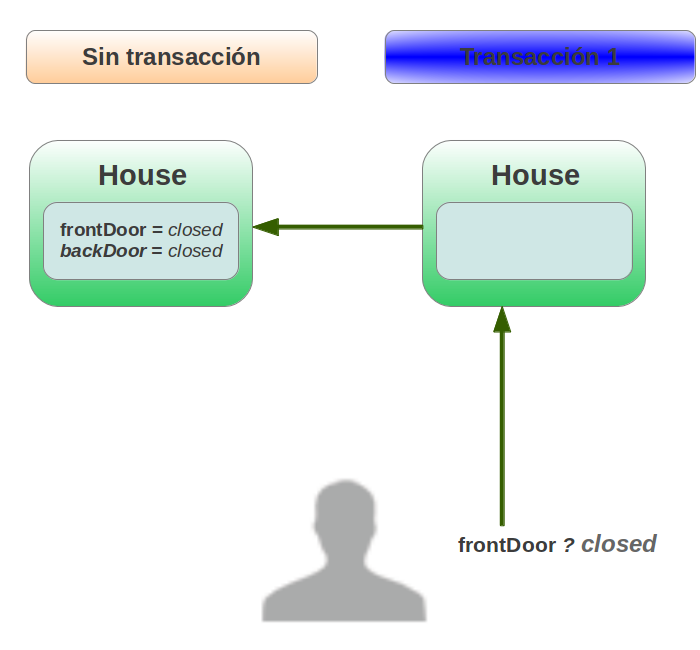
\includegraphics[scale=0.4]{img/contextoAninado1}
	    	}&
			\subfloat[Dentro del primer contexto se modifica el stock del producto, y
			ese cambio no es visible para el segundo contexto.]{
	    		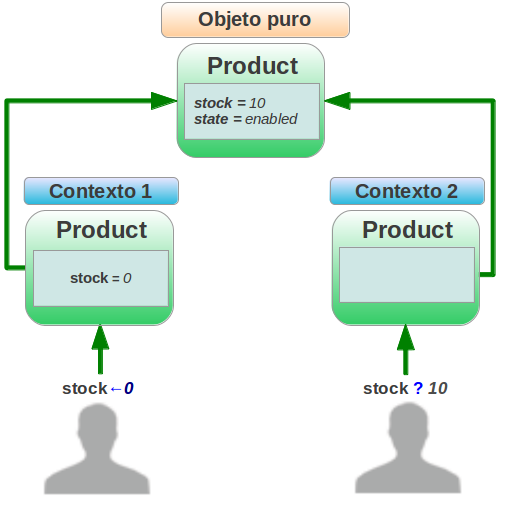
\includegraphics[scale=0.4]{img/contextoAninado2}
	    	}\\
			\subfloat[Dentro del segundo contexto se modifica el estado del producto, y
			ese cambio no es visible para el primer contexto.]{
	    		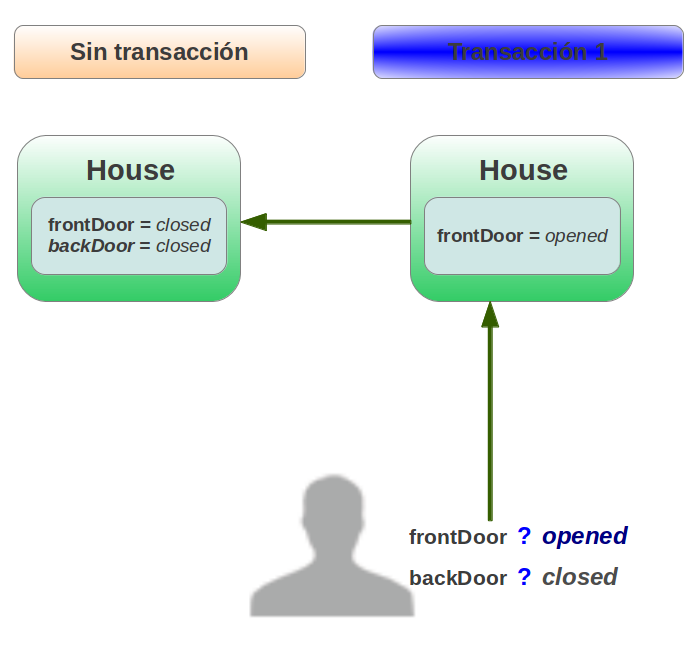
\includegraphics[scale=0.4]{img/contextoAninado3}
	    	}&
			\subfloat[El primer contexto realiza un commit confirmando sus cambios e
			impactando los mismos en el objeto; el segundo contexto se entera de esa
			modificación.]{
	    		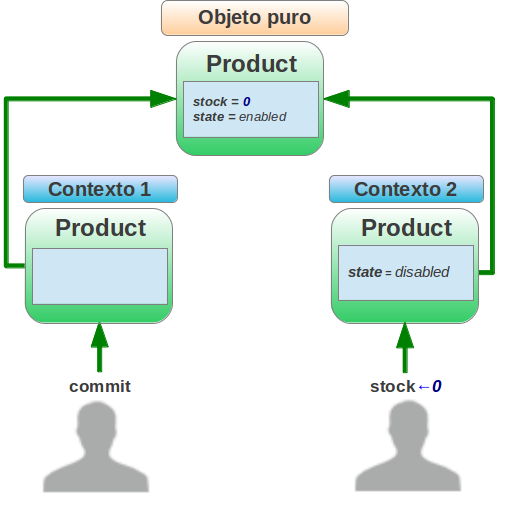
\includegraphics[scale=0.4]{img/contextoAninado4}
	    	}\\
			\subfloat[Se crea una nueva transacción anidada a la segunda.]{
	    		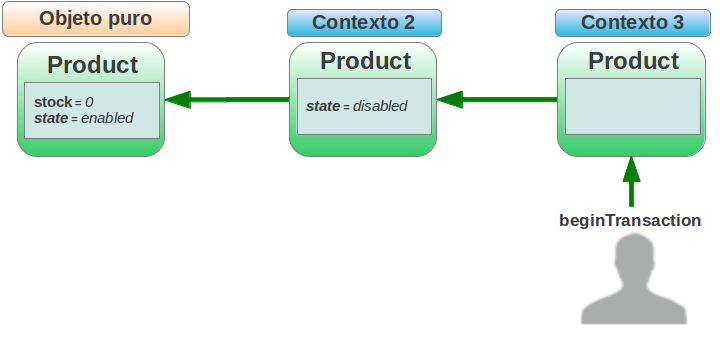
\includegraphics[scale=0.35]{img/contextoAninado5}
			}&
			\subfloat[Los cambios mutuos no son visibles fuera de su contexto.]{
	    		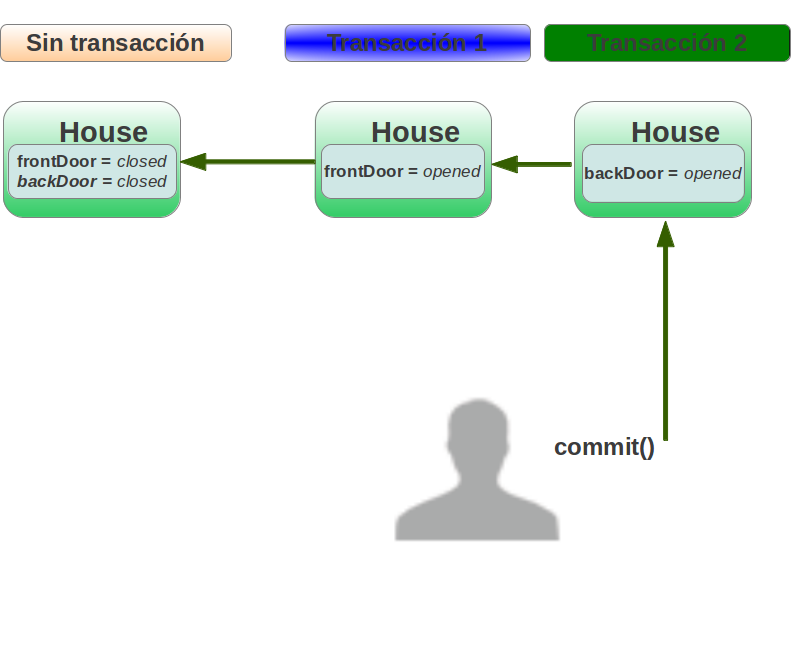
\includegraphics[scale=0.35]{img/contextoAninado6}
	    	}\\
			\subfloat[La transacción confirma sus cambios y estos son impactados
			en la transacción padre]{
	    		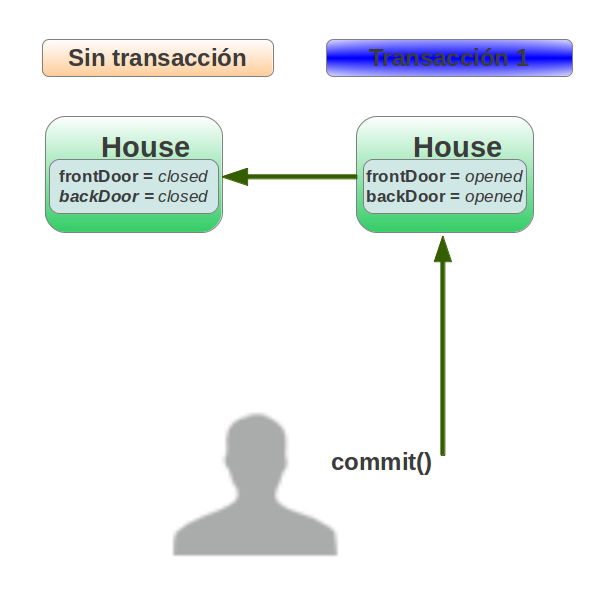
\includegraphics[scale=0.35]{img/contextoAninado7}
	    	}&
			\subfloat[La última transacción realiza un commit, y todos los cambios con
			impactados en el objeto.]{
	    		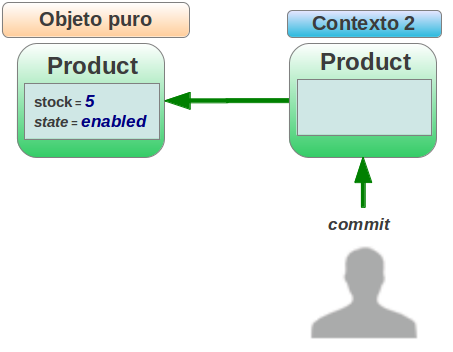
\includegraphics[scale=0.4]{img/contextoAninado8}
	    	}
			\end{tabular}
		\caption{Ejemplo del modelo transaccional}
		\label{transactionalModel}
	\end{figure}

\section{Configuración e instalación}
\label{Configuracion}
Todos los proyectos están disponibles en \url{http://xp-dev.com/svn/uqbar/projects/}.
Para más información sobre la configuración y armado del entorno de desarrollo
\url{https://sites.google.com/site/programacionui/material/herramientas/arena} y 
\url{https://www.assembla.com/wiki/show/scala-ide/With_M2Eclipse}. 






\newpage

\bibliographystyle{alpha}
\bibliography{bibliography}


\end{document}
